%\section{Introduction}
%\paragraph{Motivation: \red{ML} + Fairness}
\label{chapter:justicia}
Machine learning is becoming the omnipresent technology of our time. Machine learning classifiers are being used for high-stake decisions such as college admission~\cite{martinez2021using}, recidivism prediction~\cite{tollenaar2013method}, job applications~\cite{ajunwa2016hiring} etc. Thus, human lives are now pervasively influenced by data, classifiers, and their inherent bias.

\begin{example}\label{fairness_justicia_example:intro}
\normalfont
Let us consider an example (Figure~\ref{fairness_justicia_fig:fair_example}) of deciding the eligibility for health insurance depending on the fitness and income of individuals of different age groups (20-40 and 40-60). Typically, incomes of individuals increase as their ages increase while their fitness deteriorates. We assume that the relation of income and fitness depends on ages as per the Normal distributions in Figure~\ref{fairness_justicia_fig:fair_example}. Now, if we train a decision tree~\cite{narodytska2018learning} to decide the eligibility of an individual to get a health insurance given three features: fitness, income and age, we observe that the `optimal' decision tree (ref. Figure~\ref{fairness_justicia_fig:fair_example}) does not predict based on the sensitive feature age. However, a fairness verifier would verify that the decision tree outputs positive prediction to an individual above and below $40$ years with probabilities $0.18$ and $0.72$ respectively. This simple example demonstrates that even if a classifier does not explicitly learn to differentiate on the basis of a sensitive feature, it discriminates different age groups due to the utilitarian sense of accuracy that it tries to optimize.
\end{example}

\begin{figure}[!t]
	\centering
	\subfloat[Dependency among features and prediction]{\scalebox{1}{	
			\begin{tikzpicture}[x=1cm,y=0.6cm]
			% Define nodes
			\node[latent,scale=1] (a1) {$\textrm{age}$} ; %
			\node[obs, scale=1, below=of a1, xshift=-.8cm] (h) {$\textrm{fitness}$}; %
			\node[obs, scale=1, below=of a1, xshift=.8cm] (i) {$\textrm{income}$}; %
			\node[obs, scale=1, below=of h, xshift=.8cm] (p) {$\widehat{Y}$}; %			
			%%add edge
			\edge[] {a1} {h,i} ;
			\edge[] {h,i} {p} ;
			\end{tikzpicture}
	}}\hfil
	\subfloat[Age-dependent distributions of non-sensitive features]{
		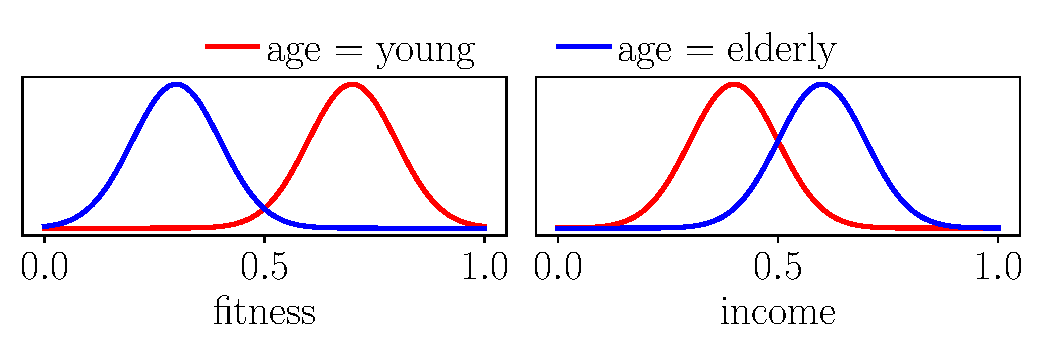
\includegraphics[scale=0.45]{figures/fairness/fif/sanity_distribution}
	}
	
	\subfloat[Trained decision tree]{
		\scalebox{0.55}{	
			\begin{tikzpicture}[x=1cm,y=1.8cm]
			\node [box, scale=1.5]                                    (p)      {fitness $\geq 0.61$};
			\node [scale=1.5, box, below= of p, xshift=-2.1cm, yshift=1.2cm]    (a1)    {income\\ $\geq 0.29$};
			\node [scale=1.5, box, below= of p, xshift=2.1cm, yshift=1.2cm]     (a2)    {income $\geq 0.69$};
			\node [scale=1.5,below= of a1, xshift=-1.5cm, yshift=0.8cm]  (a11)    { $\widehat{Y}= 1$};
			\node [scale=1.5,below= of a1, xshift=1.5cm, yshift=0.8cm]   (a12)    { $\widehat{Y}=0 $};
			\node [scale=1.5,below= of a2, xshift=-1.5cm, yshift=0.8cm]  (a21)    { $\widehat{Y}= 1$};
			\node [scale=1.5,below= of a2, xshift=1.5cm, yshift=0.8cm]  (a22)    { $\widehat{Y}= 0$};
			%
			\path [line] (p) -|         (a1) node [scale=1.5,midway, above]  {Y};
			\path [line] (p) -|         (a2) node [scale=1.5,midway, above]  {N};
			\path [line] (a1) -|       (a11) node [scale=1.5,midway, above]  {Y};
			\path [line] (a1) -|       (a12) node [scale=1.5,midway, above]  {N};
			\path [line] (a2) -|       (a21) node [scale=1.5,midway, above]  {Y};
			\path [line] (a2) -|       (a22) node [scale=1.5,midway, above]  {N};
			\end{tikzpicture}}
	}\hfil
	\subfloat[Group specific conditional probability of the classifier's positive prediction]{
		\scalebox{1}{
			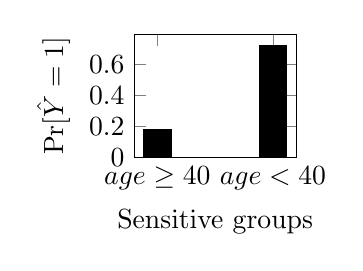
\begin{tikzpicture}
			\begin{axis}[
			enlarge x limits=0.2,
			symbolic x coords={$ \text{age} \ge 40 $, $ \text{age} < 40 $},
			xtick={$ \text{age} \ge 40 $, $ \text{age} < 40 $},  
%			xticklabel style={text height=2ex}, 
			ylabel={$ \Pr[\hat{Y} =  1] $},
			xlabel={Sensitive groups},
			ymin=0,
			width= 0.3\textwidth,] 
			
			\addplot[ybar,fill] coordinates {
				($ \text{age} \ge 40 $, 0.18)
				($ \text{age} < 40 $, 0.72)};
			
			\end{axis}
			
			\end{tikzpicture}
		}
	}
	\caption[A decision tree classifier on sensitive and non-sensitive features]{A trained decision tree to learn the eligibility for health insurance using age-dependent fitness and income indicators. This classifier makes unfair prediction to individuals with age above $ 40 $.}\label{fairness_justicia_fig:fair_example}%\vspace*{-2em}
\end{figure}


\subsubsection{Fair Machine Learning} Statistical discrimination caused by classifiers has motivated researchers to formulate several definitions of fairness and develop associated algorithms to mitigate bias. In this chapter, we focus on a popular concept of fairness, known as group fairness. Existing group fairness metrics mostly belong to three categories: \textit{independence}, \textit{separation}, and \textit{sufficiency}~\cite{mehrabi2019survey}. Independence metrics, such as demographic parity, statistical parity, and group parity, try and ensure the outcomes of a classifier to be independent of the groups that the individuals belong to~\cite{feldman2015certifying,dwork2012fairness}. Separation metrics, such as equalized odds, define a classifer to be fair if the probability of getting the same outcomes for different groups are same, separately for data from each possible ground-truth label~\cite{hardt2016equality}. Sufficiency metrics\unsure{Check definition}, such as counterfactual fairness, constrain the probability of outcomes to be independent of individual's sensitive data given their identical non-sensitive data~\cite{kusner2017counterfactual}.

In Figure~\ref{fairness_justicia_fig:fair_example}, independence is satisfied if the probability of getting insurance is same for both the age groups. Separation is satisfied if the number of `actually' (ground-truth) ineligible and eligible people getting the insurance are same. \red{Sufficiency is satisfied if the eligibility is independent of their age given their features are the same}\unsure{check}. Thus, we see that the metrics of fairness can be contradictory and complimentary depending on the application and the data~\cite{corbett2018measure}. To this end, different algorithms have also been devised to ensure one or multiple of the fairness definitions. These algorithms try to rectify and mitigate the bias in the data and thus in the classifier in three ways: \textit{pre-processing} the data~\cite{kamiran2012data,zemel2013learning,calmon2017optimized}, \textit{in-processing} the classifier~\cite{zhang2018mitigating}, and \textit{post-processing} the outcomes of a classifier~\cite{kamiran2012decision,hardt2016equality}.

\subsubsection{Fairness Verifiers} Due to the abundance of fairness metrics and difference in algorithms to achieve them, it has become necessary to verify different fairness metrics over datasets and algorithms. 

In order to verify fairness as a model property on a dataset, verifiers like \textit{FairSquare}~\cite{albarghouthi2017fairsquare} and \textit{VeriFair}~\cite{bastani2019probabilistic} have been proposed. 
%FairSquare verifies demographic parity and individual fairness as a numerical integration problem for a specific program semantics.
%VeriFair translates fairness metrics to an enumeration problem of a specified Boolean syntax.
%These papers operate for a specific Boolean sensitive feature.
These verifiers are referred to as {\em probabilistic verifiers} owing to the fact that their inputs are a probability  distribution of the features in the dataset and a classifier of a suitable form, and their objective is to verify fairness with respect to the distribution and the classifier.
Though FairSquare and VeriFair are robust and have asymptotic convergence guarantees, we observe that they scale up poorly with the size of inputs and also do not generalize to non-Boolean and compound sensitive features.
In contrast to the probabilistic verifiers, another line of work, referred to as sample-based verifiers, has focused on the design of testing methodologies  on a given fixed data sample~\cite{galhotra2017fairness,aif360-oct-2018}. 
Since sample-based verifiers are dataset-specific, they generally do not provide robustness over the distribution.


%\blue{Other papers: Probabilistic Verification of Fairness Properties via	Concentration, Verifying Individual Fairness in Machine Learning Models~\cite{john2020verifying}}
Thus, a \textit{unified formal framework} to verify \textit{different fairness metrics} of a classifer, which is \textit{scalable}, capable of \textit{handling compound protected groups}, \textit{robust} with respect to the test data, and \textit{operational on real-life} datasets and fairness-enhancing algorithms, is missing in the literature.

\subsubsection{Our Contribution.} From this vantage point, \textit{we propose to model verifying different fairness metrics as a Stochastic Boolean Satisfiability (SSAT) problem}~\cite{littman2001stochastic}. SSAT was originally introduced by ~\cite{papadimitriou1985games} to model {\em games against nature}. In this work, we primarily focus on reductions to the exist-random quantified fragment of SSAT, which is also known as E-MAJSAT~\cite{littman2001stochastic}.   SSAT is a conceptual framework that has been employed to capture several fundamental problems in artificial intelligence such as computation of maximum a posteriori (MAP) hypothesis~\cite{fremont2017maximum},  propositional probabilistic planning~\cite{majercik2007appssat},  and circuit verification~\cite{lee2018towards}. Furthermore, our choice of SSAT as a target formulation is motivated by the recent algorithmic progress that has yielded efficient SSAT tools~\cite{lee2017solving,lee2018solving}.



%We formulate SSAT encodings of the fairness verification problems and two methods to evaluate them in order to verify independence and separation metrics for any supervised learning \red{algorithm} using a unified scheme.
%Our encodings not only allow us to compute for non-Boolean and compound sensitive features but also to scale significantly better than existing formal verifiers. 
%We perform experimental analysis for multiple fairness metrics, datasets, and \red{algorithm}s to instantiate the efficiency and effectiveness of our approach.

Our contributions are summarised below:
\begin{itemize}
	\item We propose a unified SSAT-based approach, {\justicia}, to verify independence and separation metrics of group fairness and causal fairness metrics for different datasets and classifiers.
	%\item \blue{{\justicia} measures fairness metrics for pre-, in-, and post-processing \red{algorithm}s with respect to the data  generating distribution}.
	\item Unlike previously proposed formal probabilistic verifiers, namely FairSquare and VeriFair, {\justicia} verifies fairness for compound and non-Boolean sensitive features.%, and also \red{separation metrics}.
	\item Our experiments validate that our method is more accurate and scalable than the probabilistic verifiers, such as FairSquare and VeriFair, and more robust than the sample-based empirical verifiers, such as AIF360.
	\item We prove a finite-sample error bound on our estimated fairness metrics which is stronger than the existing asymptotic guarantees.
\end{itemize}

It is worth remarking that significant advances in artificial intelligence bear testimony to the right choice of formulation, for example, formulation of planning as satisfiability (SAT)~\cite{kautz1992planning}. In this context, we view that formulation of fairness as SSAT has potential to spur future work from both the modeling and encoding perspective as well as core algorithmic improvements in the underlying SSAT solvers. 

\iffalse
With this growing set of \red{algorithm}s and definitions, it has become important to measure and verify fairness and bias of different \red{algorithm}s and datasets. 
One popular approach is to use specific test dataset to compute the related statistical quantities and to certify fairness for that specific test dataset.
AIF360~\cite{aif360-oct-2018} provides a unified framework to implement multiple \red{algorithm}s and to measure their fairness depending on such test datasets.
Though this method of verification works for a specified datasets, such verifiers do not explain how much a fairness measure depends on which sensitive feature and is not robust to the selection of test dataset and its size.
\fi